\subsection{Нейронные сети}
\subsubsection{Сети прямого распространения}
\par
Целью сети прямого распространения является аппроксимация некой неизвестной функции $f$. Сеть состоит из однотипных элементов, называемых нейронами. Искусственный нейрон состоит из двух элементов: взвешенного сумматора и нелинейной функции активации над ним рис. \ref{fig:nn}.
\begin{figure}[H]
    \centering
    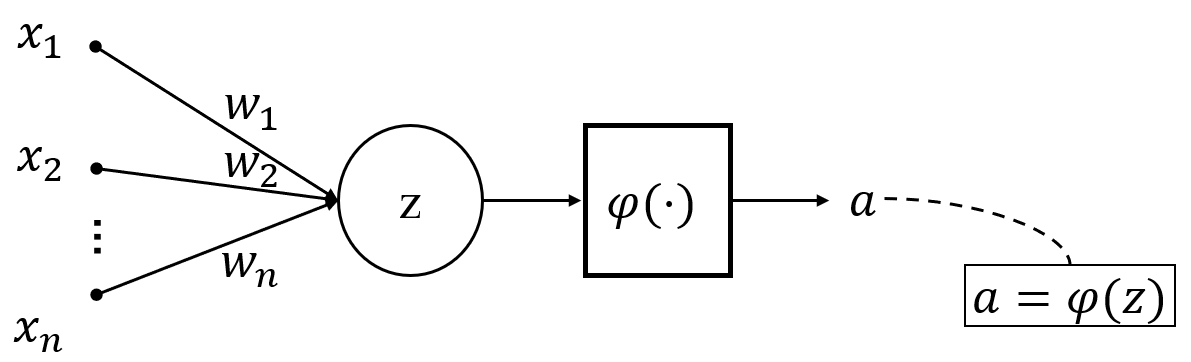
\includegraphics[scale=0.75]{nn.png}
    \caption{Модель искусственного нейрона}
    \label{fig:nn}
\end{figure}
Сумматор представляет собой выражение вида (скалярное произведение при введении $x_0 = 1$):
\[z = b + \sum\limits_{i=1}^n w_i x_i \stackrel{x_0=1}{=} w^Tx,\]
где $\vec x \in \mathbb{R}^n$ -- вектор признаков, $\vec w = \in \mathbb{R}^n$ -- вектор обучаемых параметров, $b \in \mathbb{R}$. Скопления нейронов называются слоями. Слой называется скрытым, если не определяет выход модели. Линейная композиция линейных преобразований способна представлять только линейные функции. Чтобы обобщить модель на представление нелинейных функций, вводится так называемая функция активации над результатом взвешенного сумматора. Вопрос сводится к выбору отображения. В книге \cite{Goodfellow} приведены три совета по выбору функции активации.
\subsubsection{Функции активации}
\begin{itemize}
    \item Бесконечномерная, используемая в ядерных методах (радиально-базисные) функция активации. Мощности такой функции хватит на аппроксимацию тренировочного набора, однако обобщаемость на тестовый датасет от этого страдает;
    \item Спроектировать функцию активацию $\varphi$ самостоятельно;
    \item Обучение функции активации $\varphi$. Модель представляется в несколько ином виде:
    \[y = f(x, \theta, w) = \varphi(x, \theta)^Tw.\]
    Преимуществом является выбор целого класса функций, однако придется подбирать новый гиперпараметр.
\end{itemize}
\bigskip\par 
Композиция линейных и нелинейных преобразований предоставляют универсальную аппроксимацию. Универсальная теорема аппроксимации \cite{hornik} утверждает, что сеть даже прямого распространения с линейным выходным слоем и нелинейным хотя одним слоем может аппроксимировать любую измеримую по Борелю функцию при условии, что в сети достаточно блоков. Однако эта теорема не говорит о том, насколько должна быть большой сеть. В работе \cite{barron} предпринята попытка дать верхние границы размера сети с одним уровнем -- экспоненциальное число блоков. Сети с одним слоем достаточно для универсального применения, однако этот слой может оказаться слишком большим: для решения этой проблемы под отдельные задачи берут конкретные архитектуры.

\bigskip\par 
Для классификации $n$ классов используется softmax -- функция вида:
\[\varphi(x) = \dfrac{e^{x_j}}{\sum\limits_{j=1}^Ve^{x_j}}.\]
\par
Для бинарной классификации может быть использована сигмоидная функция активации:
\[\varphi(x) = \dfrac{1}{1+e^{-x}}\]
\subsubsection{Обучение}
\par
Для обучения нейронной сети прямого распространения необходимо задать функцию ошибок между выходом сети $\tilde y$ и правильным результатом $y$. Алгоритм обратного распространения ошибки \cite{backpropagation} позволяет передавать информацию о функции ошибки обратно по сети для вычисления градиентов. Опишем граф вычисления сети прямого распространения. Пример -- граф для логистической регрессии рис. \ref{fig:logreg}:
\begin{figure}[H]
    \centering  
    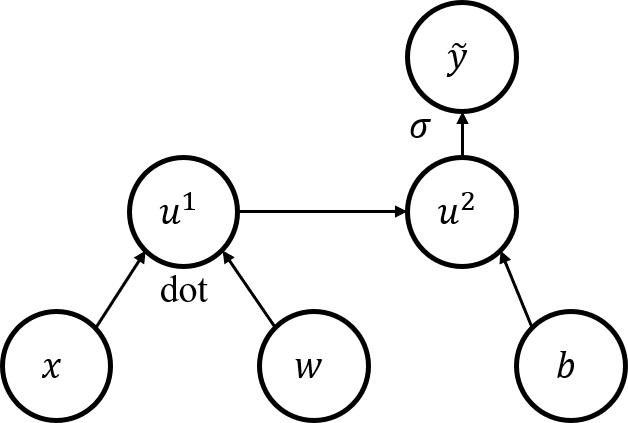
\includegraphics[scale=0.75]{log_reg.png}
    \caption{Граф вычислений для логистической регрессии}
    \label{fig:logreg}  
\end{figure}
Опишем алгоритм прохода по сети прямого распространения и вычисления функции ошибки (в общем случае с регуляризатором $\Omega(\theta)$):
\begin{algorithm}[H]
    \caption{Прямое распространение с регуляризатором $\Omega(\theta)$}\label{alg:cap}
    \begin{algorithmic}
        \State $W^{(i)}, \ i\in \left\{1, \ldots, l\right\}$
        \State $b^{(i)}, i \in \left\{1, \ldots, l\right\}$
        \State $x \gets \mathrm{input}$
        \State $y \gets \mathrm{label}$
        $s^{(0)} = x$
        \For{$k = 1, \ldots, l$}
            \State $a^{(k)} = b^{(k)} + W^{(k)}s^{(k-1)}$
            \State $s^{k} = f(a^{(k)})$
        \EndFor
        \State $\tilde y = s^{i}$
        \State $J = E(\tilde y, y) + \lambda\Omega(\theta)$
    \end{algorithmic}
\end{algorithm}
После вычисления прямого распостранения:
\begin{algorithm}[H]
    \caption{Обратное распространение ошибки}
    \label{alg:backprop}
    \begin{algorithmic}
        \State $g \gets \nabla_{\tilde y}J = \nabla_{\tilde y} E(\tilde y, y)$
        \For{$k = l, \ldots, 1$}
            \State $g\gets \nabla_{a^{(k)}}J = g \odot f'(a^{(k)})$
            \State $\text{Вычислим градиенты для смещений и весов (с регуляризацией)}$
            \State $\nabla_{b^{(k)}}J = g + \lambda\nabla_{b^{(k)}}\Omega(\theta)$
            \State $\nabla_{W^{(k)}}J = g s^{(k-1)} + \lambda\nabla_{W^{(k)}}\Omega(\theta)$

            \State $g \gets \nabla_{s^{(k-1)}}J = W^{(k)} g$
        \EndFor
    \end{algorithmic}
\end{algorithm}
Получив градиенты, можно интерпретировать эту информацию как указания о том, как следует изменить выходы слоев, чтобы уменьшить функцию ошибку. 